\chapter{Introduction}

\textit{Rendering} is generally the process of generating a 2-dimensional image, called \textit{render}, from the mathematical description of a 3-dimensional scene. 
%To oversimplify it, a scene is made of light sources, geometries and a camera, all defined in mathematical, hence rather abstract, terms. 
Several rendering algorithms have been developed over the years and many of them have been designed to produce images as \textit{photorealistic} and lifelike as possible. The most recent ones of these kind are all based upon simulating how light interacts with the scene, closely imitating its natural behavior. A particularly successful rendering algorithm following this philosophy is \textit{Path Tracing} \cite{kajiya1986rendering} since its derivation and itself are widespread across animation, visual effects and video games. In simple words, path tracing is based upon the idea of shooting rays out of an artificial camera towards the scene and make each bounce around the scene until it reaches a light source; then, the luminous energy carried by the ray and its bounces, called \textit{path}, can be computed --- or \textit{traced} back. Without even diving into its details --- which are left for section \ref{background} ---, it is clear how complex path tracing can get. This makes it difficult to grasp by people approaching it and difficult to debug.

We are presenting a tool capable to show the user an overview of the inner workings of a path tracer by providing interactive visualizations of the very core of a path tracer: paths and how they interact with the scene.
We strived to create something that does not tell but --- literally --- shows the swarm of paths shot by a path tracer to help understand what is actually going on during the rendering process.

The idea of providing interactive renderings of the data generated by a path tracer --- or a ray tracer --- is not original. Let us mention a few that inspired our work:
\begin{itemize}
	\item The \textit{Ray tracing visualization toolkit} (\textit{rtVTK}) by C. Gribble et Al. \cite{gribble2012ray} is a nice starting point but it focuses on ray tracers \cite{whitted1979improved, cook1984distributed} more than on path tracers.
	Furthermore, it is designed to render only a single ray tree at once, making it difficult to picture a global overview on the data that concurred in the generation of the final render; after all, a good mantra of presenting visual data is, quoting Ben Shneiderman, “Overview first, zoom and filter, then details-on-demand” \cite{shneiderman2003eyes}. rtVTK practically presents only the details.
	\item The work presented in \textit{A Framework for Visual Dynamic Analysis of Ray Tracing Algorithms} by H. Lesev and A. Penev \cite{lesev2014framework} has extensive filtering and data gathering features which inspired us, but it works only on ray tracers, as much as rtVTK.
	\item Another great inspiration for us was the framework presented in \textit{Applying Visual Analytics to Physically Based Rendering} by G. Simons et Al. \cite{simons2019applying}, especially the visualization parts. We however drift off it because, while they reduce the data they gather from a path tracer by selecting only about 1/6000th of the total paths, our goal is to keep the whole dataset and let the user choose what to visualize from all the samples.
	\item Another tightly related work is \textit{EMCA}, which stands for \textit{Explorer of Monte-Carlo based Algorithms}, by C. Kreisl \cite{EMCA@2019}. It focuses on path tracing and visualizations but its client-server architecture with per-pixel path analysis lacks of the global view we are trying to achieve.
\end{itemize}  

\section{Background}
\label{background}

%To fully comprehend the topics and challenges presented in this work a background is needed.

We will now provide a quick overview on path tracing to establish a common ground of terminology between us and the reader. This is not meant to be in any way an exhaustive explanation, please refer to the cited literature to have a better insight.

\subsection{The rendering equation}
\label{secrendeq}
As we introduced before, \textit{photorealistic rendering} is the process that given a mathematical description of a 3-dimensional scene outputs an as life-like as possible image, know as \textit{render}. The process simulates how light travels from light sources to an abstract camera sensor while interacting with the scene. An important equation that describes how light behaves is the \textit{Rendering Equation} introduced by J. Kajiya in 1986 \cite{kajiya1986rendering} here presented with different notations:
\begin{equation}
	L_o(\vec{x},\vec{\omega}_o) = 
		L_e(\vec{x},\vec{\omega}_o) + 
		L_r(\vec{x},\vec{\omega}_o)
	\label{rendeqeasy}
\end{equation}
It says that, considering a surface, the amount of light that leaves the surface point $\vec{x}$ in direction $\vec{\omega}_o$, called \textit{outgoing radiance} ($L_o$), is determined by the emitted radiance ($L_e$), which is the one emanated by the surface itself, plus the reflected radiance ($L_r$) which is given by:
\begin{equation}
	L_r(\vec{x},\vec{\omega}_o) = 
		\int_{\mathcal{H}^2} 
			f(\vec{\omega}_o, \vec{x}, \vec{\omega}_i)
			L_i(\vec{x},\vec{\omega}_i)
			d\vec{\omega}_i
	\label{reflectioneq}
\end{equation}
This means it consists in the sum of the radiance incoming ($L_i$) from all possible directions ($\vec{\omega}_i \in \mathcal{H}^2$) hitting point $\vec{x}$, weighted by the reflective and refractive properties of the material ($f(\cdots)$).

Now, image sensors, as well as all animal visual organs, are made of several small photo sensitive units that measure the incoming radiance hitting their surfaces over a short period of time. By putting together the values read by the units an image is produced. To compute the incoming radiance on each of these photo sensitive units called \textit{pixels}, the incoming radiance must be integrated over the pixel surface and scaled by its area to make the result independent of the sensor's size:
\begin{equation}
	L_{pixel} = \frac{1}{A_{pixel}} 
		\int_{\vec{q}\in pixel} L_i(\vec{q}, \vec{\omega}_r)dA_q
	\label{pixelradiance}
\end{equation}
Where $\vec{\omega}_r$ depends on the camera mathematical model, that can range from the simplest pinhole camera to a complex simulation of real camera lenses groups.

At this point is clear that rendering is all about computing the radiance hitting a sensor but the rendering equation presented above (eq. \ref{rendeqeasy}) describes only outgoing radiance. Fortunately, thanks to the fact that radiance is constant along a ray\footnote{Radiance is constant along a ray only in perfect vacuum. All non-volumetric path tracers --- which we exclusively focus on --- assume vacuum between surfaces.}, it is possible to write:
\begin{equation}
	L_i(\vec{x},\vec{\omega}_i) = L_o(\vec{y},\vec{\omega}_o)
\end{equation}
Where $\vec{y}$ is the first point on a surface hit by the ray shot from $\vec{x}$ in direction $\vec{\omega}_i$ and $\vec{\omega}_o$ is the direction pointing from $\vec{y}$ to $\vec{x}$. Introducing the Raytracing $RT$ operator:
\begin{equation}
	\vec{y} = RT(\vec{x},\vec{\omega}_i)
\end{equation}
And rewriting $\vec{\omega}_o$ in function of $\vec{\omega}_i$:
\begin{equation}
	\vec{\omega}_o = -\vec{\omega}_i
\end{equation}
We have that:
\begin{equation}
	L_i(\vec{x},\vec{\omega}_i) = L_o(RT(\vec{x},\vec{\omega}_i),-\vec{\omega}_i)
	\label{lilo}
\end{equation}
The first thing that can be taken from this is that to compute the incoming radiance on a sensor it is sufficient to shoot a ray and compute the radiance on the scene point hit by the ray outgoing in the inverse ray direction. Secondly, plugging everything that has been said until now produces a more complete rendering equation:
\begin{equation}
	L_o(\vec{x},\vec{\omega}_o) = 
		L_e(\vec{x},\vec{\omega}_o) + 
		\int_{\mathcal{H}^2} 
			f(\vec{\omega}_o, \vec{x}, \vec{\omega}_i)
			L_o(RT(\vec{x},\vec{\omega}_i),-\vec{\omega}_i)
			d\vec{\omega}_i
	\label{renderingeq}
\end{equation}


%Where:
%\begin{description}
%	\item[$\vec{x}$] A point in space.
%	\item[$\vec{\omega}_o$] An outgoing direction from $\vec{x}$.
%	\item[$\vec{\omega}_i$] An incoming direction towards $\vec{x}$
%	\item[$L(\vec{x},\vec{\omega}_o)$] Radiance outgoing in direction $\vec{\omega}_o$ from $\vec{x}$
%	\item[$L_e(\vec{x},\vec{\omega}_o)$] Radiance emitted in direction $\vec{\omega}_o$ by $\vec{x}$.
%	\item[$\mathcal{H}^2$] All the possible directions.
%	\item[$L(\vec{x},\vec{\omega}_i)$] Incoming radiance from direction $\vec{\omega}_i$ on $\vec{x}$.
%	\item[$f(\vec{\omega}_o, \vec{x}, \vec{\omega}_i)$] The Bidirectional Scattering Distribution Function (BSDF) computed on $\vec{x}$ on directions $\vec{\omega}_o$ and $\vec{\omega}_i$.
%	\item[$\hat{n}_{\vec{x}}$] The surface normal on $\vec{x}$.
%\end{description}

\subsection{Monte Carlo integration}

Given all the equations above, all it is needed to render a convincing image is solving them. The first problem that surfaces is that they contain integrals. Integrals are infinitesimal sums and as such they do not conform too well with the discrete nature of electronic calculators. In other words, integrals cannot be numerically solved on computers. Their solution, though, can be approximated. Without lingering on the reasons, a particularly suitable approximation method for our case is the Monte Carlo integration \cite{kalos2009monte}.

It randomly picks $N$ samples ($x_i, i \in [0,N)$) from the integration interval ($\Omega$), evaluates the integrand ($f(x)$) with each sample and does an average of the evaluated values weighting them by the probability density function ($pdf(x)$) of picking the corresponding sample from the interval. This gives:
\begin{equation}
	\int_{\Omega}f(x)dx \approx \frac{1}{N} \sum_{i=0}^{N} \frac{f(x_i)}{pdf(x_i)}
	\label{montecarlo}
\end{equation}

The value computed by Monte Carlo gets closer to the correct result increasing the number of random samples $N$. It has been demonstrated that if the samples are picked from the interval using a uniform distribution, the relative error is directly proportional to $\frac{1}{\sqrt{N}}$. From this it can be deducted that Monte Carlo will never output the correct solution but it will asymptotically tend to it as samples increase; that is why literature usually talk about \textit{convergence} and sometimes about \textit{convergence speed}, which is an informal value expressing how many samples are needed to approximate an acceptable result, where what is considered acceptable varies case by case.

The $\frac{1}{\sqrt{N}}$ factor can be improved by a technique called \textit{importance sampling} that is based upon the idea of drawing samples from a distribution as close as possible to the integrand in order to reduce the variance. The ideal case would be using the integrand itself as distribution but often, due to its complexity, is impossible to draw samples directly from it. Alternative distributions that roughly approximate the integrand are used instead.
This can even be brought a step forward by stochastically combining two approximate distributions together using the so-called \textit{multiple importance sampling} (MIS) \cite{veach1995optimally}.

\subsection{Path tracing}

Now that we have a tool to numerically solve integrals, we can apply it to the integrals presented in section \ref{secrendeq}. The total incoming radiance on a pixel (eq. \ref{pixelradiance}) can then be calculated by randomly picking sample points on its surface and then applying Monte Carlo (eq. \ref{montecarlo}):
\begin{equation}
	L_{pixel} \approx \frac{1}{N A_{pixel}} 
		\sum^{N}_{i = 0} \frac{L_i(\vec{q}_i, \vec{\omega}_{ri})}{p(\vec{q}_i)}
\end{equation}
The number of samples picked here $N$ is usually constant for each pixel. Due to its direct relation between final render quality --- more samples means a solution closer to the real one --- and render time --- each additional sample adds computational burden --- it is a rather important parameter in all path tracers and it is called \textit{samples per pixel} or \textit{spp} for short.

Now, it is a matter of computing $L_i$ for each pixel sample. Recalling the logical results given by the conservation of radiance along rays presented in equation \ref{lilo} the problem shifts on how to compute the outgoing radiance of the point of the scene hit by the ray shot from the sample position ($\vec{q}_i$) in its associated direction ($\vec{\omega}_{ri}$). This value, as presented by the complete version of the rendering equation (eq. \ref{renderingeq}), depends on another integral having all possible directions as its integration interval. Furthermore, inside the integral there is again an outgoing radiance, but this time computed with other parameters ($L_o(RT(\vec{x},\vec{\omega}_i),-\vec{\omega}_i)$). By substitution, it begins to become clear that evaluating one outgoing radiance theoretically leads to solving a recursively infinite amount of integrals. This, through the power of Monte Carlo integration, becomes manageable and a path tracer computes outgoing radiances by sampling all the possible directions just once. The rendering equation can then be written as:
\begin{equation}
	L_o(\vec{x},\vec{\omega}_o) \approx
	L_e(\vec{x},\vec{\omega}_o) + 
	\frac{1}{pdf(\vec{\omega}_i)}
	f(\vec{\omega}_o, \vec{x}, \vec{\omega}_i)
	L_o(RT(\vec{x},\vec{\omega}_i),-\vec{\omega}_i)	
\end{equation}
With this approximation the calculations consist in shooting a ray, find an intersection with the scene, compute the properties of the material on the intersection, pick a random new direction, shoot a ray in that direction from the intersection point and then keep doing the same recursively, forming a path. In practice, to not make a path bounce indefinitely, a maximum number of bounces, called \textit{maximum path length}, is arbitrarily decided before rendering, as much as the number of samples per pixel is.

Path tracers that behave as described until now are informally called na\"ive path tracers. Other more complex tracers employ techniques to speed up the Monte Carlo convergence. As already mentioned, a common technique is importance sampling, as it can be applied to path tracing by sampling new bounces' directions from probability distributions that naturally carry more radiance. This can happen in two ways: either paths are forced to follow the properties of the material they are bouncing on, or they are directed towards a light source. A usually even more efficient approach is to combine these two sampling strategies through multiple importance sampling.

% Using this approximation, estimating radiance for each pixel sample can be written in pseudo code as shown in listing \ref{ptalgo}.
% It is clear how 

% \begin{Listing}
% 	\begin{lstlisting}
% function estimate_radiance(ray):
% 	intersection := intersect scene with ray
% 	if no intersection:
% 		return 0

% 	x := intersection point
% 	omega_o := ray direction
% 	omega_i := random direction picked from distribution d
% 	pdf_omega_i := pdf of the distribution d evaluated for omega_i
% 	new_ray := ray originating from x and direction omega_i
% 	incoming_radiance := estimate_radiance(new_ray)
% 	material := material properties computed with omega_o, x, and omega_i
% 	return (1 / pdf_omega_i) * material * incoming_radiance

% primary_ray := ray shot from the camera
% estimate_radiance(primary_ray)
% 	\end{lstlisting}
% 	\caption{Pixel sample radiance estimation.}
% 	\label{ptalgo}
% \end{Listing}

%\subsection{OpenGL}



%It means that the algorithms that generated these datasets have different ways of choosing the direction of each path bounce in order to maximize the radiance carried by each path, speeding up the convergence of the Monte Carlo integration and hence trying to lower the amount of noise given the same amount of pixel samples. This technique, used in every application of Monte Carlo methods, is called \textit{importance sampling} \cite{kalos2009monte}. Multiple importance sampling \cite{veach1995optimally}.

\section{Motivation}
\label{motivation}
%As introduced above, path tracing is an algorithm that is not easy to picture. For someone who got to understand it, the rendering equation is more than enough to tell how a path tracer work. At least to get started, everything a person needs to know is in that equation: once combined with Monte Carlo integration, everyone is theoretically ready to implement a path tracer. 

As introduced above, path tracing is not easy to picture. As many research groups before us thought, having a tool showing what a tracer is doing by visualizing its interactions with the 3d scene would help the professional developers lost in the debugging cycle as well as the students trying to get a hang of path tracing's inner workings. The challenge this vision has to face is the sheer amount of these interactions; talking about path tracing, to have a decent render\footnote{We considered as a decent render a $512 \times 512$ pixels and 256 spp image which is a good halfway point between production quality and being way too far from convergence.}, more than two hundreds paths have to be shot for each pixel: to produce an image, more than fifty million paths have to be shot. Postponing data size considerations for later (sec. \ref{datatogather}), leaves us with potential datasets that without proper data reduction or filtering are of no use to anyone. Related works usually perform substantial reductions of the datasets \cite{simons2019applying,EMCA@2019}, but we believe that having all the paths available to visualization would improve the experience.

With these premises, a more precise idea for a visualization tool came to us. 
The user should have the power to visually and interactively explore all the paths previously generated by a path tracer during rendering. The paths have to be immersed in an interactive rendering of the scene: their most important property is their geometry or, in other words, where they bounce inside the scene. Even if out of curiosity and naivety we tried visualizing all the paths of smaller datasets achieving compelling yet cluttered results (fig. \ref{visual_clutter}), visualizing the millions of paths all together was out of question since the beginning. To navigate this ocean of paths, the user should be provided with a global summary overview of the dataset in its entirety, and they should also able to filter them using spatial queries. For the global overview we envisioned a heatmap applied as a texture to the 3d view of the scene that shows areas where there is more path activity, while for the spatial queries we thought the user might want to select path bouncing on certain noteworthy surfaces, such as lights or mirrors. 

\begin{figure}
	\centering
	\centering
	\begin{subfigure}[t]{0.49\linewidth}
		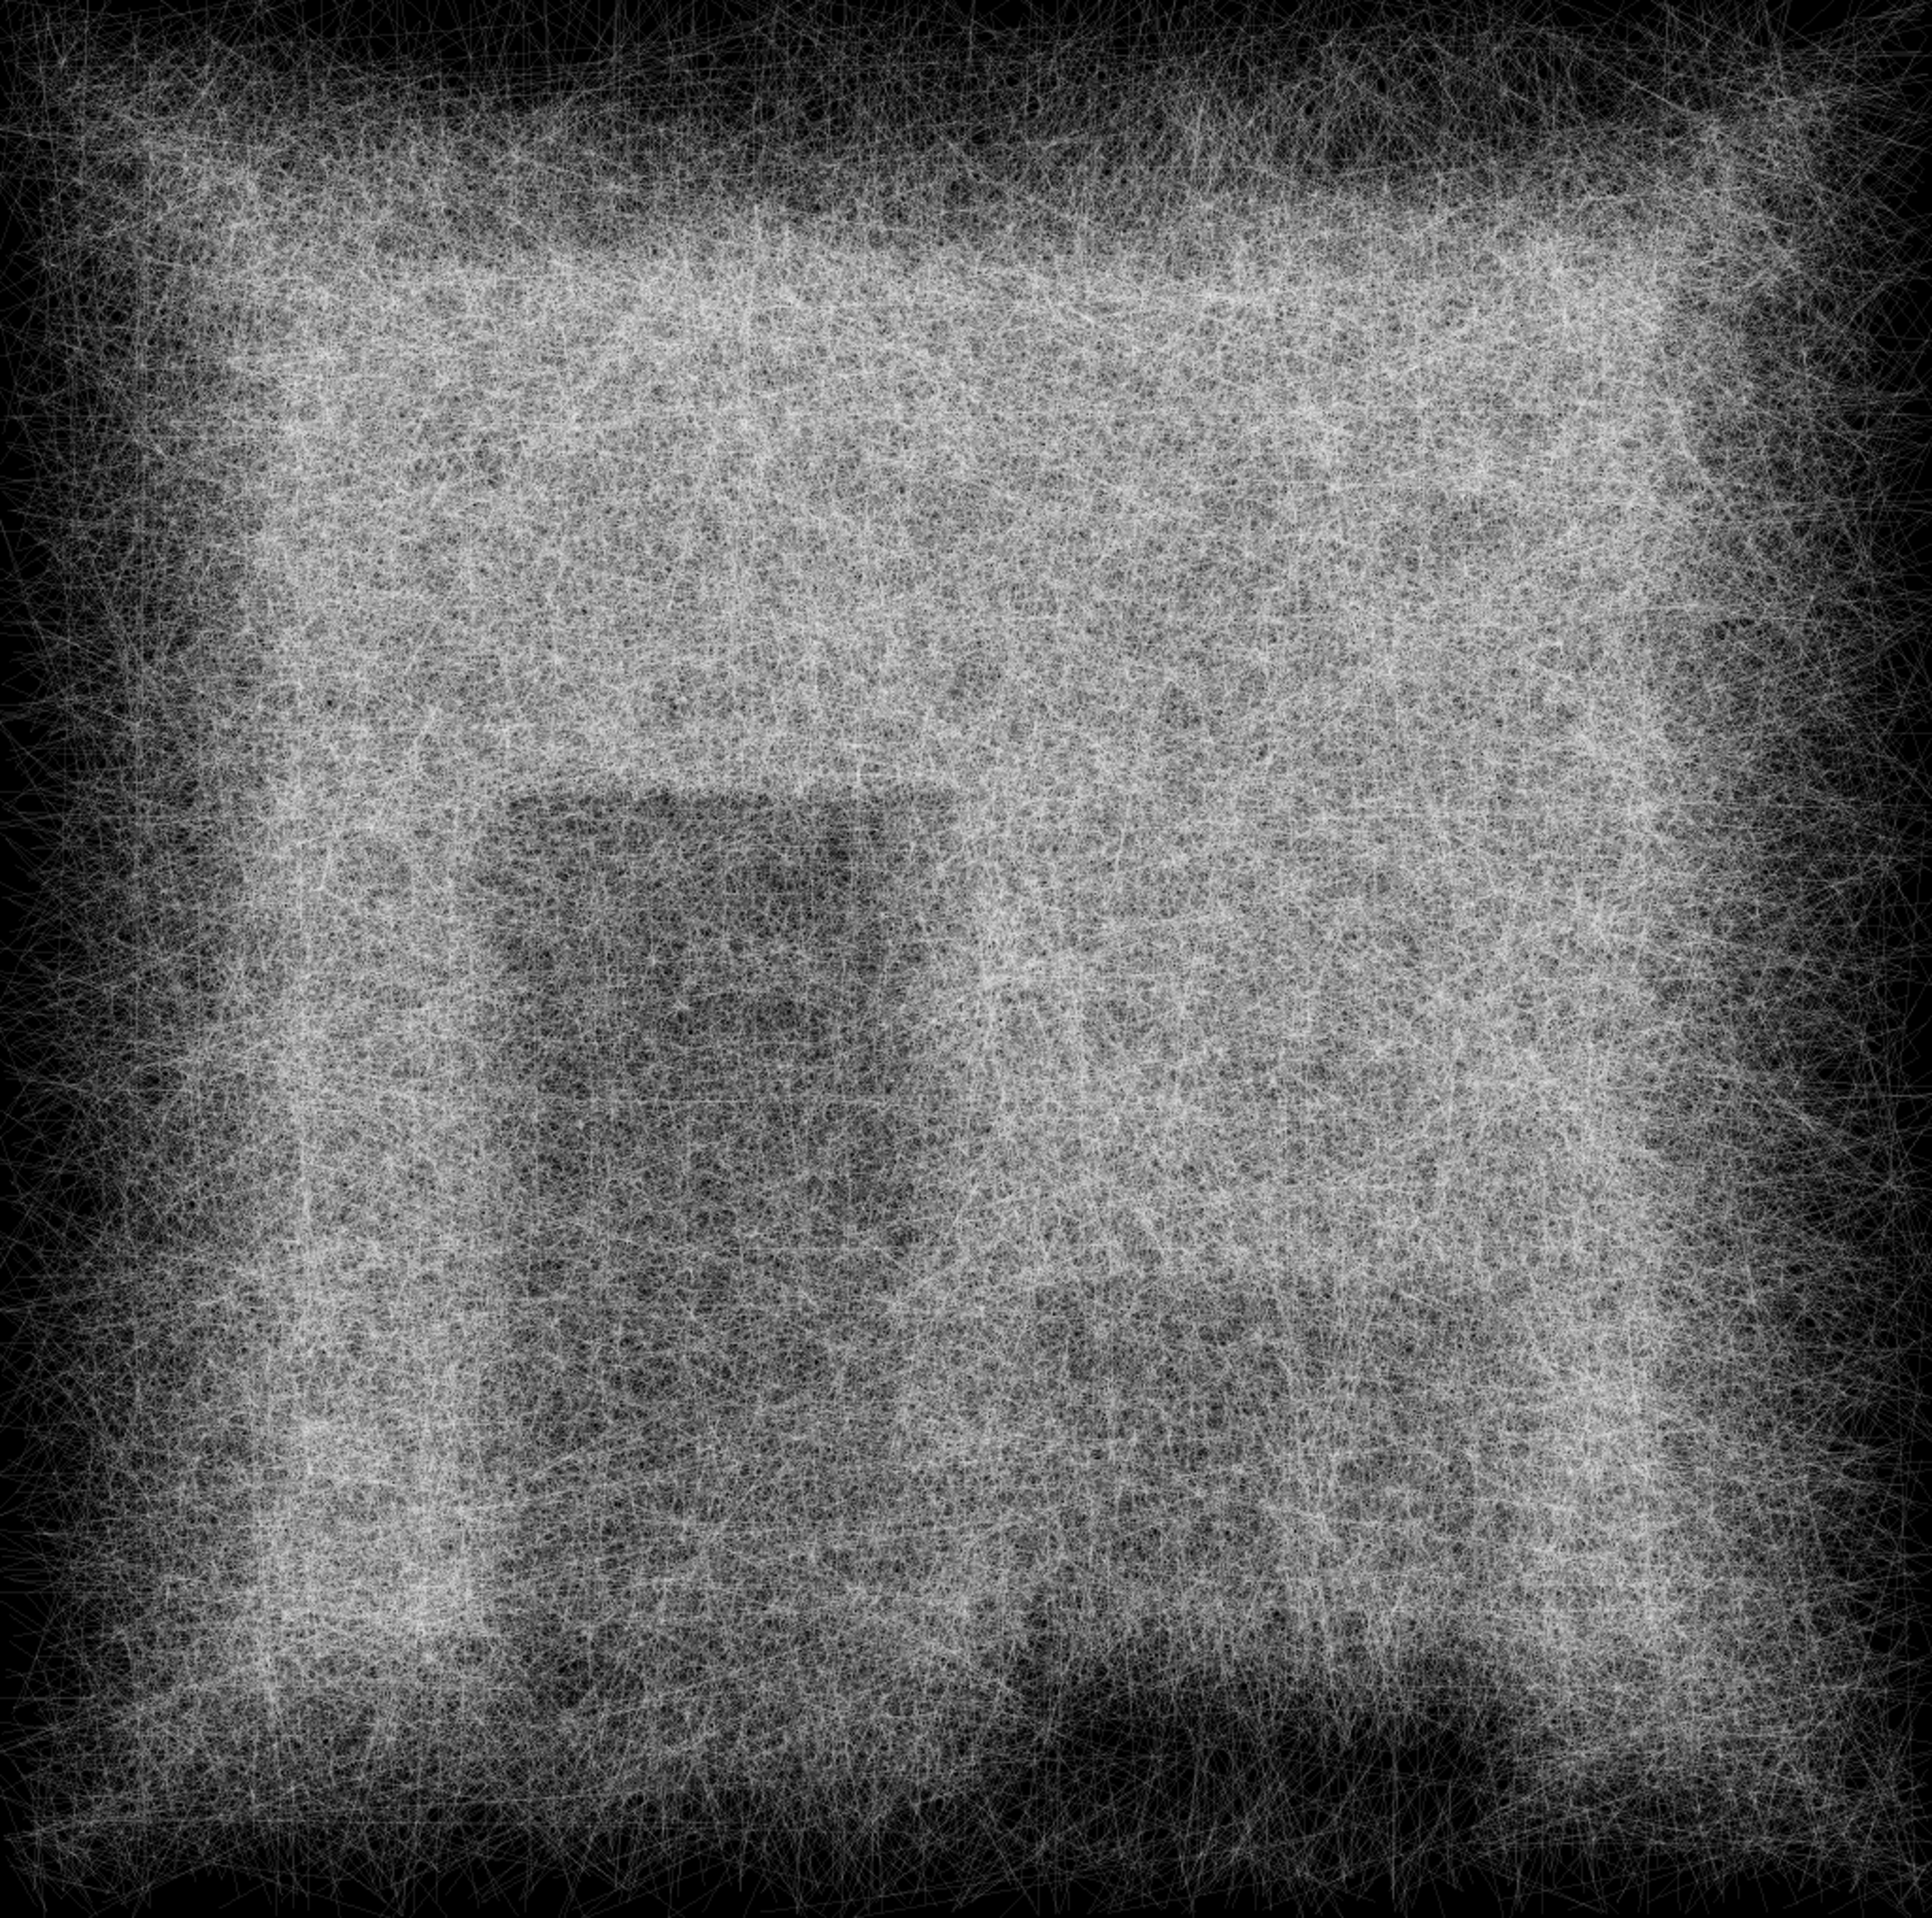
\includegraphics[width=\textwidth]{chapters/chapter_intro/clutter_early1}
		\caption{$64 \times 64$, 1 spp}
	\end{subfigure}
	\begin{subfigure}[t]{0.49\linewidth}
		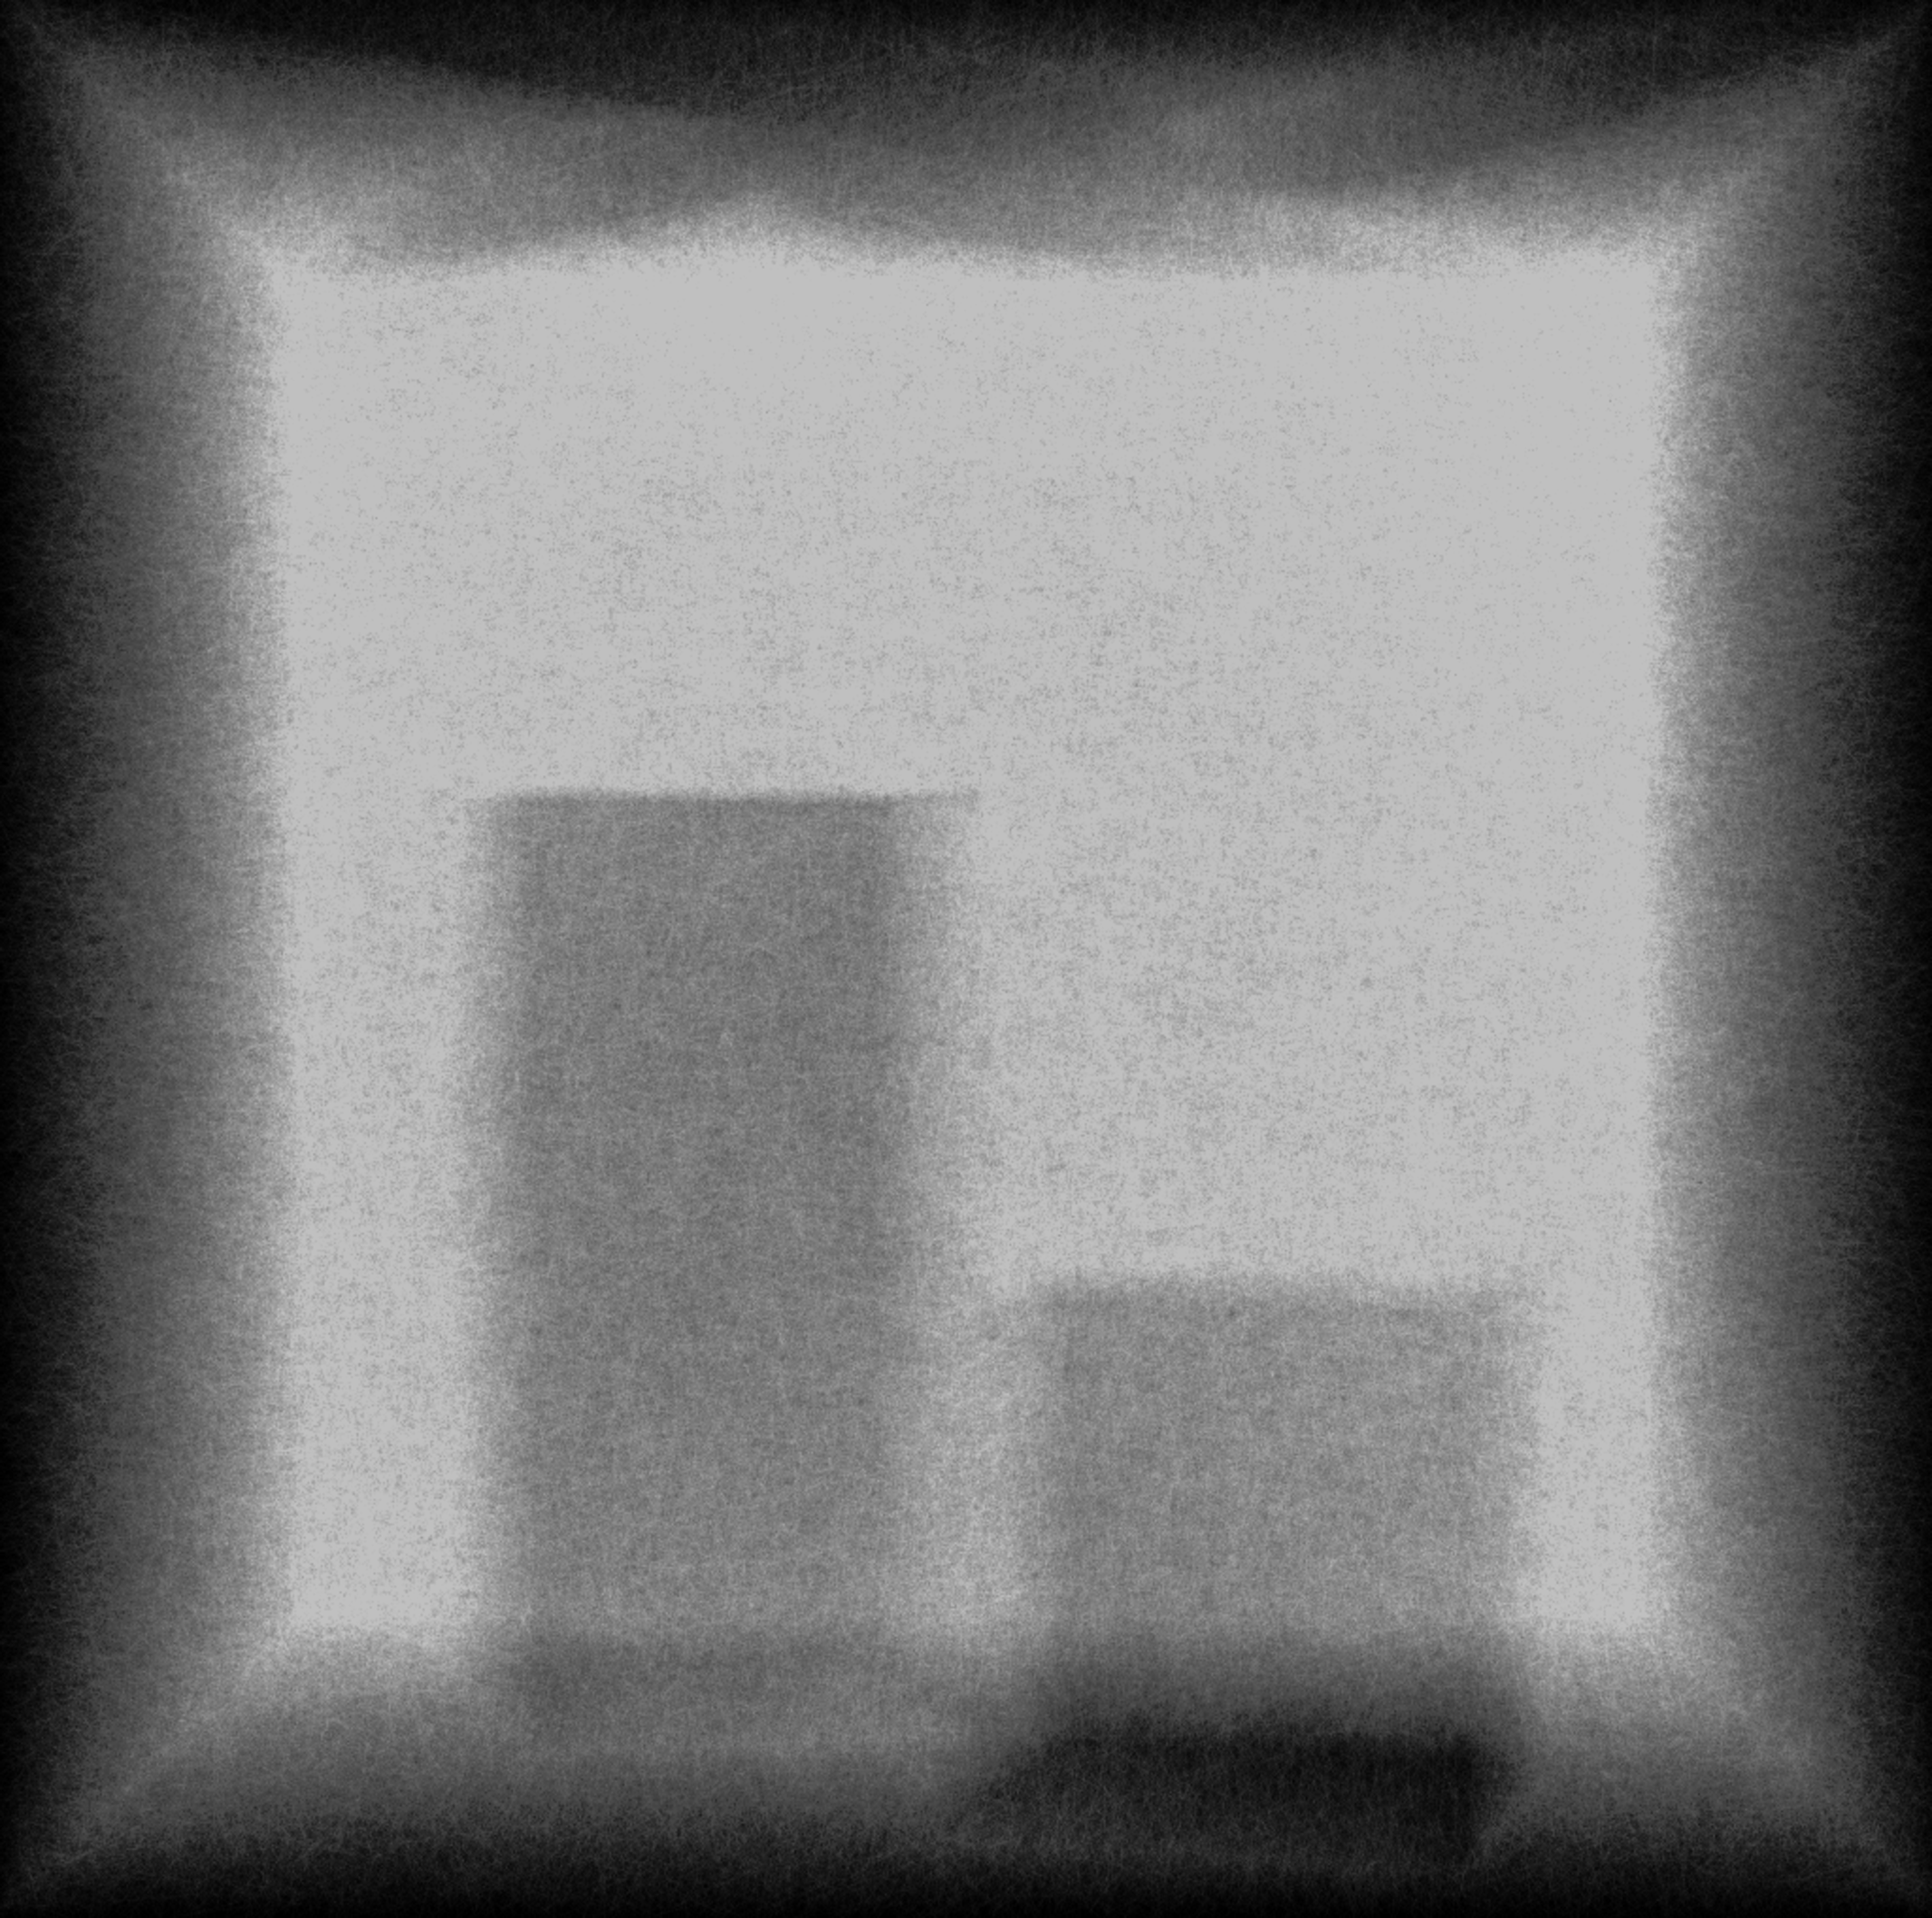
\includegraphics[width=\textwidth]{chapters/chapter_intro/clutter_early2}
		\caption{$64 \times 64$, 64 spp}
	\end{subfigure}
	
	\caption{Visual clutter in an early version of the tool where the scene rendering has not been implemented yet. Both datasets have been generated on the \textit{Cornell Box} scene.}
	\label{visual_clutter}
\end{figure}

Later in the development, it became clear that the possibility of comparing different datasets would come in handy to users. It could be useful in many cases such as comparing two progressive versions of the same in-development path tracer to understand what changed or, more in an educational context, such as showing a ground truth next to a purposely wrong dataset to understand why one is wrong on a deeper level.

Of course, before even talking about visualizing data, data has to be gathered from a path tracer. We envisioned a software piece, parallel to the visualization client, able to plug to any path tracer and gather with little effort the required data during the rendering process. Then the idea of a gathering library with a very simple interface came about; a library that can be plugged into any path tracer the user is currently working on by just calling the few required functions.

To summarize, our vision consisted in a tool divided into a visualization client and a data gathering library which can be used both for debugging and teaching purposes. The library should have an easy to interact with interface, while the client would let the user explore different datasets simultaneously and in their entirety using the filtering and visualization options provided to them.

%select a portion of a surface of the 3d scene the tracer has been run upon and see the paths that bounce there with a bunch of useful data. To be able to do that the whole set of paths shoot by a tracer are needed: by the very stochastic nature of a path tracer, it is impossible to determine which paths will end up bouncing where without resolving them all first. That is why it has been decided it was essential to store data about each path during the rendering process. To make the tool usable in most possible use cases, it had to be able to plug into an existing path tracer and this lead to the conception of the tool as a two software pieces suite: a \textit{data gatherer library} called \texttt{gatherer} and a \textit{visualization client} called \texttt{gathererclient}.

%Now this “useful data” was not extremely well-defined during those early stages, so most of the efforts have been directed to the very essential: rendering the requested paths keeping interactivity.